\chapter{Client-side Prediction \& Reconciliation}
Im folgenden Abschnitt werden die im Projekt umgesetzten und verwendeten Mechaniken beschrieben und anhand des Quellcode beschrieben.
Hierbei liegt der Fokus darauf, ein durchdachtes System zu verwenden, das den Kern der Problematik einfach im Spiel erkenntlich machen kann. 

\section{Client-side Prediction beim Bewegen und Schießen}

In einem serverautoritativen Netzwerkmodell ist es essenziell, ein faires und sicheres Spielumfeld zu gewährleisten. Gleichzeitig darf die Spielbarkeit aus Sicht des Spielers nicht unter einer hohen Latenz leiden. Besonders bei reaktionsintensiven Genres wie First-Person-Shootern oder Rennspielen ist eine direkte Rückmeldung auf Eingaben entscheidend für das Spielerlebnis.

Ein vollständiger Verzicht auf Client-Authorität würde zwar maximale Sicherheit bieten, jedoch zu spürbarer Verzögerung bei der Bewegung oder Aktion führen. Ziel ist daher ein Kompromiss: Der Server behält die Entscheidungsgewalt, während der Client Eingaben sofort lokal umsetzt und visuelles Feedback liefert.

\newpage
In der vorliegenden Implementierung wird dies durch ein Überschreiben der Unity-eigenen \texttt{NetworkTransform}-Komponente realisiert. Die Autoritätslogik wird über eine einfache Enumeration gesteuert:

\lstinputlisting[
  style=csharpStyle,
  caption={Überschreiben der NetworkTransform-Komponente mit AuthorityMode},
  label={lst:authority-mode} 
]{src/PlayerMovement/ClientNetworkTransform.cs}


Die Methode \texttt{OnIsServerAuthoritative()} gibt in der Regel \texttt{false} zurück, sodass der Client die Kontrolle über Bewegung und Eingabe erhält, ohne dass ein Roundtrip zum Server erforderlich ist. Dadurch wird die Latenzwahrnehmung beim Spieler erheblich reduziert.


\newpage
\section{Reconciliation – Zustandskorrektur  bei Abweichungen}

Trotz lokaler Vorhersage durch den Client bleibt der Server die Referenzinstanz für den „wahren“ Spielzustand. Sollte es zu größeren Abweichungen zwischen Client- und Serverposition kommen, wird ein Reconciliation-Prozess ausgelöst. Dabei wird der Client zurück auf den zuletzt vom Server bestätigten Zustand gesetzt und die eigenen Eingaben ab diesem Zeitpunkt erneut simuliert.

In Spielen mit präzisem Bewegungsfeedback (z.B. FPS) ist die Toleranzschwelle für Positionsfehler oft sehr gering. In diesem Projekt wurde ein Grenzwert: \\ (\texttt{reconciliationThreshold}) definiert, ab dem eine Zustandskorrektur erfolgt. Dieser Wert kann abhängig von variabler Netzwerklatenz angepasst werden.

\begin{figure}[H] % oder [htbp]
    \centering
    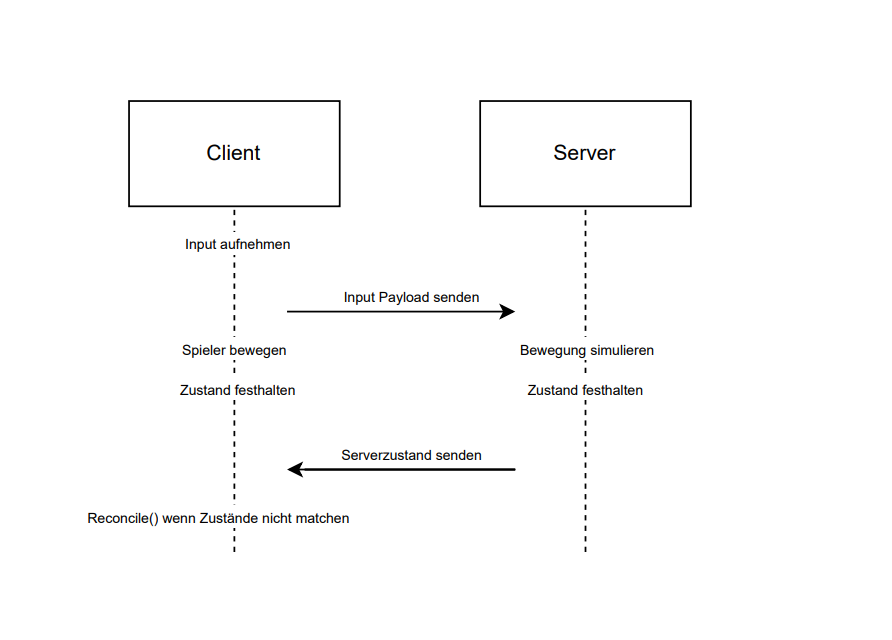
\includegraphics[width=0.8\textwidth]{figures/ReconciliationSeq.png}
    \caption{Sequenzdiagramm Reconciliation}
    \label{fig:logo}
\end{figure}

\section{Testmechanismus zur Validierung}

Zur gezielten Auslösung der Reconciliation wurde ein einfacher Testmechanismus implementiert: Ein Client-Cheat teleportiert den Spieler um 20 Einheiten nach vorne – weit über die Fehlertoleranz hinaus. Der Server erkennt die Abweichung und triggert die Korrektur, wodurch der Spieler sichtbar in den korrekten Zustand „zurückspringt“.

Zur Visualisierung wurden farblich unterschiedliche Proxies (3D-Würfel) über dem Spielerobjekt angezeigt, die die vom Client bzw. Server berechneten Zustände darstellen.

\section{Datenstrukturen und Ticksystem}
Als Datenstruktur wurde für das Ticksystem auf zirkuläre Buffer gesetzt. Im Netcode-Bereich ist dies defacto Standard <Quelle maybe> um die mit den einzelnen Ticks verbundenen Informationen oder genauer Positionen, Rotationen und Geschwindigkeiten umzugehen und Overheads zu negieren.
Demnach eignen sich bspw. Arrays oder Dictionaries deutlich schlechter, da diese die gespeicherten Informationen nicht verwerfen und somit unnöitge Daten halten, die für bspw. die Reconciliation außer Reichweite liegen und somit die Performance beeinträchtigen.
In Kombination mit State und Input Payloads die jeweils als Structs implementiert wurden, sollen die Positionen zum passenden Tick verglichen werden können.
Die Eigenimplementierung des Circular Buffer ist somit generisch und basiert auf den Input oder State Payloads. Mit der Methode Add(), die ein generisches Item also in diesem Fall das State oder Input Payload und einen Index als Parameter nimmt, kann somit der Buffer befüllt werden.
Das Befüllen folgt den algorithmischen Grundlagen eines solchen Buffers und das geschieht bis zu der statischen Buffergröße und fängt dann wieder von null an zu indezieren. 
Somit werden in diesem Fall intern also bis 1024 Ticks verwaltet, was bei einer Standard-Tickrate von 60Hz ungefähr 17 Sekunden wären, die man zurückspulen könnte.
Eine solche Buffergröße ist im Grunde schon relativ großzügig, sollte man jedoch auf eine Tickbasis aufsteigen von etwa 128Hz, ist es schon etwas sinnvoller.  (vielleicht noch erwähnen warum genau...) 

\newpage

Im Folgenden sieht man noch den Aufbau des Circular Buffers und die Strukturen die essentiell sind für den Datentransfer:
\lstinputlisting[
  style=csharpStyle,
  caption={Methode \texttt{CircularBuffer()}},
  label={lst:circular-buffer}
]{src/CircularBuffer.cs}

\newpage
Auf der anderen Seite muss dies durch die angesprochenen Strukturen gespeichert werden:
\lstinputlisting[
  style=csharpStyle,
  caption={Methode \texttt{Payload}},
  label={lst:payload}
]{src/Payload.cs}
In der InputPayload werden die Eingabedaten des Spielers verwaltet und serialisiert, was über die vom zu implementierenden Interface INetworkSerializeable gestellten Methode NetworkSerialize() getan wird.

\section{Kernmethoden der Reconciliation-Logik}
Im Grunde lässt sich die Logik auf einige Methoden runterbrechen, dies sich alle im PlayerMovement Skript befinden. Diese Methoden sind jedoch verschachtelt in einem komplexeren Ablauf dieses Skriptes, reichen aber fürs Verständnis aus. 
\newpage
\begin{enumerate}
    \item \texttt{ShouldReconcile()} \\
    Diese Methode prüft, ob neue Serverdaten vorliegen und ob diese sich vom zuletzt verarbeiteten Zustand unterscheiden:

\lstinputlisting[
  style=csharpStyle,
  caption={Methode \texttt{ShouldReconcile()}},
  label={lst:should-reconcile}
]{src/PlayerMovement/ShouldReconcile.cs}

    \item \texttt{ReconcileState(StatePayload rewindState)} \\
    Hier wird der Client-Zustand auf den vom Server bestätigten Zustand zurückgesetzt. Anschließend werden alle seitdem aufgezeichneten Eingaben erneut angewendet:

\lstinputlisting[
  style=csharpStyle,
  caption={Methode \texttt{ReconcileState(StatePayload)}},
  label={lst:reconcile-state}
]{src/PlayerMovement/ReconcileState.cs}

    \item \texttt{HandleServerReconciliation()} \\
    Diese Methode koordiniert den gesamten Reconciliation-Prozess und vergleicht die Zustände beider Seiten:

\lstinputlisting[
  style=csharpStyle,
  caption={Methode \texttt{HandleServerReconciliation()}},
  label={lst:handle-server-reconciliation}
]{src/PlayerMovement/HandleServerReconciliation.cs}